% Options for packages loaded elsewhere
\PassOptionsToPackage{unicode}{hyperref}
\PassOptionsToPackage{hyphens}{url}
\PassOptionsToPackage{dvipsnames,svgnames,x11names}{xcolor}
%
\documentclass[
  letterpaper,
  DIV=11,
  numbers=noendperiod]{scrartcl}

\usepackage{amsmath,amssymb}
\usepackage{lmodern}
\usepackage{setspace}
\usepackage{iftex}
\ifPDFTeX
  \usepackage[T1]{fontenc}
  \usepackage[utf8]{inputenc}
  \usepackage{textcomp} % provide euro and other symbols
\else % if luatex or xetex
  \usepackage{unicode-math}
  \defaultfontfeatures{Scale=MatchLowercase}
  \defaultfontfeatures[\rmfamily]{Ligatures=TeX,Scale=1}
\fi
% Use upquote if available, for straight quotes in verbatim environments
\IfFileExists{upquote.sty}{\usepackage{upquote}}{}
\IfFileExists{microtype.sty}{% use microtype if available
  \usepackage[]{microtype}
  \UseMicrotypeSet[protrusion]{basicmath} % disable protrusion for tt fonts
}{}
\makeatletter
\@ifundefined{KOMAClassName}{% if non-KOMA class
  \IfFileExists{parskip.sty}{%
    \usepackage{parskip}
  }{% else
    \setlength{\parindent}{0pt}
    \setlength{\parskip}{6pt plus 2pt minus 1pt}}
}{% if KOMA class
  \KOMAoptions{parskip=half}}
\makeatother
\usepackage{xcolor}
\usepackage[top=30mm,left=30mm,heightrounded]{geometry}
\setlength{\emergencystretch}{3em} % prevent overfull lines
\setcounter{secnumdepth}{-\maxdimen} % remove section numbering
% Make \paragraph and \subparagraph free-standing
\ifx\paragraph\undefined\else
  \let\oldparagraph\paragraph
  \renewcommand{\paragraph}[1]{\oldparagraph{#1}\mbox{}}
\fi
\ifx\subparagraph\undefined\else
  \let\oldsubparagraph\subparagraph
  \renewcommand{\subparagraph}[1]{\oldsubparagraph{#1}\mbox{}}
\fi

\usepackage{color}
\usepackage{fancyvrb}
\newcommand{\VerbBar}{|}
\newcommand{\VERB}{\Verb[commandchars=\\\{\}]}
\DefineVerbatimEnvironment{Highlighting}{Verbatim}{commandchars=\\\{\}}
% Add ',fontsize=\small' for more characters per line
\usepackage{framed}
\definecolor{shadecolor}{RGB}{241,243,245}
\newenvironment{Shaded}{\begin{snugshade}}{\end{snugshade}}
\newcommand{\AlertTok}[1]{\textcolor[rgb]{0.68,0.00,0.00}{#1}}
\newcommand{\AnnotationTok}[1]{\textcolor[rgb]{0.37,0.37,0.37}{#1}}
\newcommand{\AttributeTok}[1]{\textcolor[rgb]{0.40,0.45,0.13}{#1}}
\newcommand{\BaseNTok}[1]{\textcolor[rgb]{0.68,0.00,0.00}{#1}}
\newcommand{\BuiltInTok}[1]{\textcolor[rgb]{0.00,0.23,0.31}{#1}}
\newcommand{\CharTok}[1]{\textcolor[rgb]{0.13,0.47,0.30}{#1}}
\newcommand{\CommentTok}[1]{\textcolor[rgb]{0.37,0.37,0.37}{#1}}
\newcommand{\CommentVarTok}[1]{\textcolor[rgb]{0.37,0.37,0.37}{\textit{#1}}}
\newcommand{\ConstantTok}[1]{\textcolor[rgb]{0.56,0.35,0.01}{#1}}
\newcommand{\ControlFlowTok}[1]{\textcolor[rgb]{0.00,0.23,0.31}{#1}}
\newcommand{\DataTypeTok}[1]{\textcolor[rgb]{0.68,0.00,0.00}{#1}}
\newcommand{\DecValTok}[1]{\textcolor[rgb]{0.68,0.00,0.00}{#1}}
\newcommand{\DocumentationTok}[1]{\textcolor[rgb]{0.37,0.37,0.37}{\textit{#1}}}
\newcommand{\ErrorTok}[1]{\textcolor[rgb]{0.68,0.00,0.00}{#1}}
\newcommand{\ExtensionTok}[1]{\textcolor[rgb]{0.00,0.23,0.31}{#1}}
\newcommand{\FloatTok}[1]{\textcolor[rgb]{0.68,0.00,0.00}{#1}}
\newcommand{\FunctionTok}[1]{\textcolor[rgb]{0.28,0.35,0.67}{#1}}
\newcommand{\ImportTok}[1]{\textcolor[rgb]{0.00,0.46,0.62}{#1}}
\newcommand{\InformationTok}[1]{\textcolor[rgb]{0.37,0.37,0.37}{#1}}
\newcommand{\KeywordTok}[1]{\textcolor[rgb]{0.00,0.23,0.31}{#1}}
\newcommand{\NormalTok}[1]{\textcolor[rgb]{0.00,0.23,0.31}{#1}}
\newcommand{\OperatorTok}[1]{\textcolor[rgb]{0.37,0.37,0.37}{#1}}
\newcommand{\OtherTok}[1]{\textcolor[rgb]{0.00,0.23,0.31}{#1}}
\newcommand{\PreprocessorTok}[1]{\textcolor[rgb]{0.68,0.00,0.00}{#1}}
\newcommand{\RegionMarkerTok}[1]{\textcolor[rgb]{0.00,0.23,0.31}{#1}}
\newcommand{\SpecialCharTok}[1]{\textcolor[rgb]{0.37,0.37,0.37}{#1}}
\newcommand{\SpecialStringTok}[1]{\textcolor[rgb]{0.13,0.47,0.30}{#1}}
\newcommand{\StringTok}[1]{\textcolor[rgb]{0.13,0.47,0.30}{#1}}
\newcommand{\VariableTok}[1]{\textcolor[rgb]{0.07,0.07,0.07}{#1}}
\newcommand{\VerbatimStringTok}[1]{\textcolor[rgb]{0.13,0.47,0.30}{#1}}
\newcommand{\WarningTok}[1]{\textcolor[rgb]{0.37,0.37,0.37}{\textit{#1}}}

\providecommand{\tightlist}{%
  \setlength{\itemsep}{0pt}\setlength{\parskip}{0pt}}\usepackage{longtable,booktabs,array}
\usepackage{calc} % for calculating minipage widths
% Correct order of tables after \paragraph or \subparagraph
\usepackage{etoolbox}
\makeatletter
\patchcmd\longtable{\par}{\if@noskipsec\mbox{}\fi\par}{}{}
\makeatother
% Allow footnotes in longtable head/foot
\IfFileExists{footnotehyper.sty}{\usepackage{footnotehyper}}{\usepackage{footnote}}
\makesavenoteenv{longtable}
\usepackage{graphicx}
\makeatletter
\def\maxwidth{\ifdim\Gin@nat@width>\linewidth\linewidth\else\Gin@nat@width\fi}
\def\maxheight{\ifdim\Gin@nat@height>\textheight\textheight\else\Gin@nat@height\fi}
\makeatother
% Scale images if necessary, so that they will not overflow the page
% margins by default, and it is still possible to overwrite the defaults
% using explicit options in \includegraphics[width, height, ...]{}
\setkeys{Gin}{width=\maxwidth,height=\maxheight,keepaspectratio}
% Set default figure placement to htbp
\makeatletter
\def\fps@figure{htbp}
\makeatother

\KOMAoption{captions}{tableheading}
\makeatletter
\makeatother
\makeatletter
\makeatother
\makeatletter
\@ifpackageloaded{caption}{}{\usepackage{caption}}
\AtBeginDocument{%
\ifdefined\contentsname
  \renewcommand*\contentsname{Table of contents}
\else
  \newcommand\contentsname{Table of contents}
\fi
\ifdefined\listfigurename
  \renewcommand*\listfigurename{List of Figures}
\else
  \newcommand\listfigurename{List of Figures}
\fi
\ifdefined\listtablename
  \renewcommand*\listtablename{List of Tables}
\else
  \newcommand\listtablename{List of Tables}
\fi
\ifdefined\figurename
  \renewcommand*\figurename{Figure}
\else
  \newcommand\figurename{Figure}
\fi
\ifdefined\tablename
  \renewcommand*\tablename{Table}
\else
  \newcommand\tablename{Table}
\fi
}
\@ifpackageloaded{float}{}{\usepackage{float}}
\floatstyle{ruled}
\@ifundefined{c@chapter}{\newfloat{codelisting}{h}{lop}}{\newfloat{codelisting}{h}{lop}[chapter]}
\floatname{codelisting}{Listing}
\newcommand*\listoflistings{\listof{codelisting}{List of Listings}}
\makeatother
\makeatletter
\@ifpackageloaded{caption}{}{\usepackage{caption}}
\@ifpackageloaded{subcaption}{}{\usepackage{subcaption}}
\makeatother
\makeatletter
\@ifpackageloaded{tcolorbox}{}{\usepackage[many]{tcolorbox}}
\makeatother
\makeatletter
\@ifundefined{shadecolor}{\definecolor{shadecolor}{rgb}{.97, .97, .97}}
\makeatother
\makeatletter
\makeatother
\ifLuaTeX
  \usepackage{selnolig}  % disable illegal ligatures
\fi
\IfFileExists{bookmark.sty}{\usepackage{bookmark}}{\usepackage{hyperref}}
\IfFileExists{xurl.sty}{\usepackage{xurl}}{} % add URL line breaks if available
\urlstyle{same} % disable monospaced font for URLs
\hypersetup{
  colorlinks=true,
  linkcolor={blue},
  filecolor={Maroon},
  citecolor={Blue},
  urlcolor={Blue},
  pdfcreator={LaTeX via pandoc}}

\author{}
\date{}

\begin{document}
\ifdefined\Shaded\renewenvironment{Shaded}{\begin{tcolorbox}[boxrule=0pt, borderline west={3pt}{0pt}{shadecolor}, frame hidden, sharp corners, breakable, interior hidden, enhanced]}{\end{tcolorbox}}\fi

\setstretch{1.2}
\hypertarget{vm303-01-studies-in-digital-media-culture}{%
\subsection{VM303-01 Studies in Digital Media \&
Culture}\label{vm303-01-studies-in-digital-media-culture}}

\begin{figure}

\begin{minipage}[t]{0.49\linewidth}

{\centering 

\raisebox{-\height}{

\href{https://opensea.io/assets/ethereum/0xdfde78d2baec499fe18f2be74b6c287eed9511d7/14000027}{\includegraphics{img/minipods.gif}}

}

\caption{}

}

\end{minipage}%
%
\begin{minipage}[t]{0.02\linewidth}

{\centering 

~

}

\end{minipage}%
%
\begin{minipage}[t]{0.49\linewidth}

{\centering 

\href{https://emerson.edu/academics/academic-departments/visual-media-arts}{Department
of Visual \& Media Arts}\\
\href{https://emerson.edu/}{Emerson College}\\
Spring Semester 2023\\
Tues/Thur 17 January---4 May 2023 6:00-7:45 p.m.\\
Ansin 605\\
\href{http://mroberts.emerson.build/}{Dr.~Martin Roberts}\\
Office hrs: Thur 3:00-5:00 p.m.\\
Office: Ansin 915C\\

}

\end{minipage}%

\end{figure}

\begin{center}\rule{0.5\linewidth}{0.5pt}\end{center}

\href{https://mroberts.emerson.build/courses/vm-303-01/sp23/}{Syllabus}
(outside Canvas) \textbar{}
\href{https://canvas.emerson.edu/courses/1932613/pages/mastodon-quickstart}{Mastodon
Quickstart}
\textbar~\href{https://mroberts1.github.io/wordcloud}{Wordcloud}

\begin{center}\rule{0.5\linewidth}{0.5pt}\end{center}

\begin{Shaded}
\begin{Highlighting}[]
\NormalTok{P5 = require("p5")}
\NormalTok{function* createSketch(sketch) \{}
\NormalTok{  const element = DOM.element(\textquotesingle{}div\textquotesingle{});}
\NormalTok{  yield element;}
\NormalTok{  const instance = new P5(sketch, element, true);}
\NormalTok{  try \{}
\NormalTok{    while (true) \{}
\NormalTok{      yield element;}
\NormalTok{    \}}
\NormalTok{  \} finally \{}
\NormalTok{    instance.remove();}
\NormalTok{  \}}
\NormalTok{\}}
\NormalTok{class Dot \{}
\NormalTok{  constructor(sketch, x, y, colour, size) \{}
\NormalTok{    this.s = sketch;}
\NormalTok{    this.x = x | 0;}
\NormalTok{    this.y = y | 0;}
\NormalTok{    this.colour = colour;}
\NormalTok{    this.size = size;}
\NormalTok{    this.velX = this.s.random({-}2, 2);}
\NormalTok{    this.velY = this.s.random({-}2, 2);}
\NormalTok{  \}}
\NormalTok{  on() \{}
\NormalTok{    this.s.noStroke();}
\NormalTok{    this.s.fill(this.colour);}
\NormalTok{    this.s.circle(this.x, this.y, this.size);}
\NormalTok{  \}}
\NormalTok{  move() \{}
\NormalTok{    this.x += this.velX;}
\NormalTok{    this.y += this.velY;}
\NormalTok{  \}}
  
\NormalTok{  bounce(radius, inside) \{}
\NormalTok{    let x = this.x {-} this.s.width/2;}
\NormalTok{    let y = this.y {-} this.s.height/2;}
\NormalTok{    if (}
\NormalTok{      inside \&\& x*x + y*y \textgreater{} radius * radius ||}
\NormalTok{      !inside \&\& x*x + y*y \textless{} radius * radius}
\NormalTok{    ) \{}
    
\NormalTok{      // https://math.stackexchange.com/a/611836}
\NormalTok{      let nx = x / this.s.sqrt(x*x + y*y);}
\NormalTok{      let ny = y / this.s.sqrt(x*x + y*y);}
\NormalTok{      let vx = this.velX;}
\NormalTok{      let vy = this.velY;}
\NormalTok{      this.velX = (ny*ny {-} nx*nx)*vx {-} 2*nx*ny*vy;}
\NormalTok{      this.velY = (nx*nx {-} ny*ny)*vy {-} 2*nx*ny*vx;}
    
\NormalTok{    \}}
\NormalTok{  \}}
  
\NormalTok{\}}
\NormalTok{createSketch(s =\textgreater{} \{}
\NormalTok{  let n = 100;}
\NormalTok{  let dot;}
\NormalTok{  let dotList = [];}
\NormalTok{  let palette = [}
\NormalTok{    s.color("\#6B1B00"),}
\NormalTok{    s.color("\#AE8B70"),}
\NormalTok{    s.color("\#F9FEFB"),}
\NormalTok{    s.color("\#56382D") }
\NormalTok{  ];}
\NormalTok{  s.setup = function() \{}
\NormalTok{    s.createCanvas(746, 746);}
\NormalTok{    for(let i = 0; i \textless{} n; i++) \{}
\NormalTok{      let angle = s.random(0, s.TWO\_PI);}
\NormalTok{      let radius = s.width * s.random(.12, .33);}
\NormalTok{      dotList.push(dot = new Dot(}
\NormalTok{        s,}
\NormalTok{        s.width/2 + s.cos(angle) * radius,}
\NormalTok{        s.height/2 + s.sin(angle) * radius,}
\NormalTok{        s.random(palette),}
\NormalTok{        s.random(1, 5)}
\NormalTok{      ));}
\NormalTok{    \}}
\NormalTok{  \};}
    
\NormalTok{  s.draw = function() \{}
\NormalTok{    dotList.map(dot =\textgreater{} \{}
\NormalTok{      dot.on();}
\NormalTok{      dot.move();}
\NormalTok{      dot.bounce(s.width * .35, true);}
\NormalTok{      dot.bounce(s.width * .1, false);}
\NormalTok{    \});}
\NormalTok{  \};}
\NormalTok{\})}
\end{Highlighting}
\end{Shaded}

\textbf{Breaking News} more at 6

2023-05-04\_Thur
\href{https://mroberts1.github.io/wordcloud/}{Wordcloud}

2023-05-04\_Thur
\href{https://www.politico.eu/article/artificial-intelligence-technology-art-regulation-copyright/}{The
New Luddites}

2023-05-02\_Tues \href{https://jan.bot/livelog}{JAN BOT\_ RIP}

2023-05-02\_Tues
\href{https://huggingface.co/spaces/huggingface-projects/stable-diffusion-multiplayer}{Stable
Diffusion Multiplayer}

2023-05-02\_Tues
\href{https://www.youtube.com/watch?v=PJlvf5rM3Hg}{Talkin' 'bout my
generation}

2023-04-25\_Tues
\href{https://dokoissho.sdf.org/conferences/moving-targets/}{Moving
Targets: Object Detection \& Algorithmic Aesthetics}

2023-04-25\_Tues
\href{https://podcasts.apple.com/us/podcast/humans-vs-machines-with-gary-marcus/id1532110146}{\emph{Humans
vs.~Machines}} (new AI podcast hosted by Gary Marcus)

2023-04-25\_Tues
\href{https://medium.com/@socialcreature/ai-and-the-american-smile-76d23a0fbfaf}{AI
and the American Smile}

2023-04-20\_Thur
\href{https://www.buzzfeednews.com/article/chrisstokelwalker/ai-hip-hop-rap-music-drake-kanye-weeknd-rihanna-jay-z?fbclid=IwAR2GilfS-1q_2ZzhA-JgJawRULmSc2tcSATLVEri1Ux8SDDcmY9rTKy1ClY}{Fake
Drakes and Counterfeit Kanyes}

2023-04-20\_Thur \href{https://research.runwayml.com/gen2}{Gen-2: The
Next Step Forward for Generative AI}

2023-04-20\_Thur \href{https://itch.io/jams}{Game Jams}

2023-04-18\_Tues
\href{https://garymarcus.substack.com/p/stop-treating-ai-models-like-people}{Stop
Treating AI Models Like People}

2023-04-18\_Tues \href{https://operationalimages.cz/}{Operational
Images}

2023-04-18\_Tues
\href{https://jussiparikka.net/2022/02/16/operational-images-preface-in-the-forthcoming-book/}{Preface:
Operational Images, All the Way Down}

2023-04-06\_Thur

\href{https://day1.postphotography.xyz/}{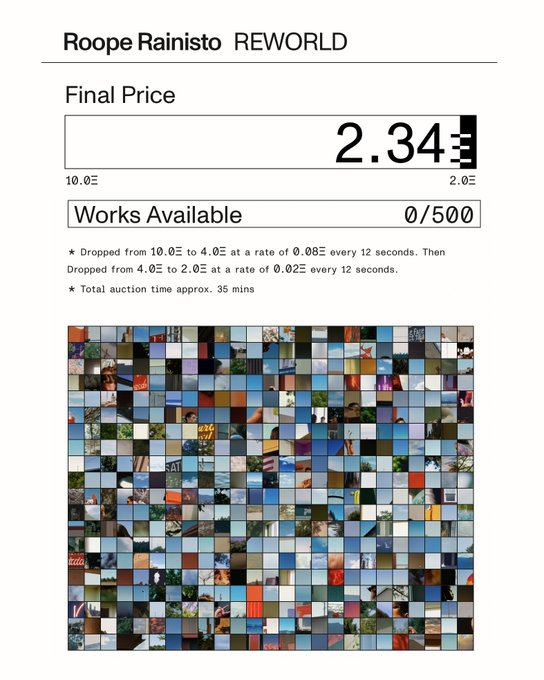
\includegraphics{img/rr-auction.jpg}}{]}

2023-04-06\_Thur
\href{https://twitter.com/Historic_Crypto/status/1641106531147030530}{Twitter
thread on post-photography}

2023-04-04\_Tues \href{https://postphotography.xyz/}{Post-Photographic
Perspectives}

2023-03-30\_Thur \href{https://artofthebrickexhibit.com/}{The Art of the
Brick}

2023-03-30\_Thur
\href{https://kotaku.com/steam-pc-ai-generated-art-midjourney-youtube-valve-1849531585}{Kotaku
article on AI-generated Steam games}

2023-03-30\_Thur
\href{https://garymarcus.substack.com/p/the-open-letter-controversy}{Gary
Marcus post on the two links below}

2023-03-30\_Thur
\href{https://twitter.com/garymarcus/status/1641137676618457088?s=46\&t=0Inx0sRD_78X35N9VmpoqA}{Twitter
thread on alternatives to the Open Letter AI moratorium}

2023-03-30\_Thur
\href{https://twitter.com/GaryMarcus/status/1641420433391259648}{Gary
Marcus Twitter longread about the Open Letter controversy}

2023-03-28\_Tues
\href{https://futureoflife.org/open-letter/pause-giant-ai-experiments/}{Pause
Giant AI Experiments: An Open Letter}

\begin{center}\rule{0.5\linewidth}{0.5pt}\end{center}



\end{document}
